\chapter{Quickstart}
\label{chap:quickstart}
\index{quickstart}

This chapter demonstrates how to get started with \dolfin{}, including
downloading and installing the latest version of \dolfin{}, and solving
Poisson's equation. These topics are discussed in more detail
elsewhere in this manual. In particular, see
Appendix~\ref{app:installation} for detailed installation instructions
and Chapter~\ref{sec:pde} for a detailed discussion of how to solve
partial differential equations with \dolfin{}.

%------------------------------------------------------------------------------
\section{Downloading and installing \dolfin{}}
\index{downloading}
\index{installation}

The latest version of \dolfin{} can be found on the \fenics{} web page:
\begin{code}
  http://www.fenics.org/
\end{code}
The following commands illustrate the installation process, assuming
that you have downloaded release 0.1.0 of \dolfin{}:
\begin{code}
  # tar zxfv dolfin-0.1.0.tar.gz
  # cd dolfin-0.1.0
  # ./configure
  # make
  # make install
\end{code}

Note that you may need to be root on your system to perform the last
step.\footnote{To install \dolfin{} locally on a normal user account,
configure \dolfin{} to use another installation directory, for example
\texttt{./configure --prefix=\~{}/local}. Alternatively, you may use the
command \texttt{./configure.local} to install \dolfin{} locally in a
subdirectory of the source tree.}  Since \dolfin{} depends on a number
of other packages, you may also need to download and install these
packages before you can compile \dolfin{}.  (See
Appendix~\ref{app:installation} for detailed instructions.)

%------------------------------------------------------------------------------
\section{Solving Poisson's equation with \dolfin{}}
\index{Poisson's equation}

Let's say that we want to solve Poisson's equation on the unit square
$\Omega = (0,1) \times (0,1)$ with homogeneous Dirichlet boundary
conditions on the boundary $\Gamma_0 = \{(x, y) \in \partial \Omega : x = 0\}$,
the Neumann boundary condition $\partial_n u = 1$ on the boundary $\Gamma_1 = \{(x, y) \in \partial \Omega : x = 1\}$,
homogeneous Neumann boundary conditions on the remaining part of the boundary
and right-hand side given by $f(x, y) = 500 \exp(-((x-0.5)^2 +
(y-0.5)^2)/0.02)$, corresponding to a source localized at $x = y = 0.5$:
\begin{eqnarray} \label{eq:poisson,quickstart}
  - \Delta u(x, y) &=& f(x, y), \quad
  x \in \Omega = (0,1) \times (0,1), \\
  u(x, y) &=& 0, \quad
  (x, y) \in \Gamma_0 = \{(x, y) \in \partial \Omega : x = 0\}, \\
  \partial_n u(x, y) &=& 1, \quad
  (x, y) \in \Gamma_1 = \{(x, y) \in \partial \Omega : x = 1\}, \\
  \partial_n u(x, y) &=& 0, \quad
  (x, y) \in \partial \Omega \setminus (\Gamma_0 \cup \Gamma_1).
\end{eqnarray}

To solve a partial differential equation with \dolfin{}, it must first
be rewritten in \emph{variational form}.  The (discrete) variational
formulation of Poisson's equation reads: Find $U \in V_h$ such that
\begin{equation} \label{eq:varform}
  a(v, U) = L(v) \quad \forall v\in \hat{V}_h, 
\end{equation}
with $(\hat{V}_h, V_h)$ a pair of suitable discrete function spaces
(the test and trial spaces). The bilinear form $a : \hat{V}_h \times V_h
\rightarrow \R$ is given by
\begin{equation}
  a(v, U) = \int_{\Omega} \nabla v \cdot \nabla U \dx
\end{equation}
and the linear form $L : \hat{V}_h \rightarrow \R$ is given by
\begin{equation}
  L(v) = \int_{\Omega} v f \dx + \int_{\partial \Omega} v g \ds,
\end{equation}
where $g = \partial_n u$ is the Neumann boundary condition.

\subsection{Setting up the variational formulation}
\index{ffc}

The variational formulation (\ref{eq:varform}) must be given to
\dolfin{} as a pair of bilinear and linear forms $(a, L)$ using the
form compiler \ffc{}. This is done by entering the definition of
the forms in a text file with extension \texttt{.form},
e.g. \texttt{Poisson.form}, as follows:
\begin{code}
  element = FiniteElement(``Lagrange'', ``triangle'', 1)

  v = TestFunction(element)
  U = TrialFunction(element)
  f = Function(element)
  g = Function(element)
  
  a = dot(grad(v), grad(U))*dx
  L = v*f*dx + v*g*ds
\end{code}

The example is given here for piecewise linear finite elements in two
dimensions, but other choices are available, including arbitrary order
Lagrange elements in two and three dimensions.

To compile the pair of forms $(a, L)$, now call the form compiler on
the command-line as follows:
\begin{code}
  # ffc Poisson.form
\end{code}
This generates the file \texttt{Poisson.h} which implements the forms
in C++ for inclusion in your \dolfin{} program.

\subsection{Writing the solver}

Having compiled the variational formulation (\ref{eq:varform})
with \ffc{}, it is now easy to implement a solver for Poisson's
equation. We first discuss the implementation line by line and then
present the complete program. The source code for this example is
available in the directory \texttt{src/demo/pde/poisson/} of the \dolfin{}
source tree.

At the beginning of our C++ program, which we write in a text file
named \texttt{main.cpp}, we must first include the header file
\texttt{dolfin.h}, which gives our program access to the \dolfin{}
class library. In addition, we include the header file
\texttt{Poisson.h} generated by the form compiler. Since all classes
in the \dolfin{} class library are defined within the namespace
\texttt{dolfin}, we also specify that we want to work within this
namespace:
\begin{code}
  #include <dolfin.h>
  #include ``Poisson.h''
  
  using namespace dolfin;
\end{code}

Since we are writing a C++ program, we need to create a \texttt{main}
function.  You are free to organize your program any way you like, but
in this simple example we just write our program inside the
\texttt{main} function:

\begin{code}
  int main()
  \{
    // Write your program here
    return 0;
  \}
\end{code}

We now proceed to specify the right-hand side $f$ of (\ref{eq:poisson,quickstart}).
This is done by defining a new subclass of \texttt{Function}
and overloading the \texttt{eval()}
function to return the value $f(x, y) = 500 \exp(-((x-0.5)^2 +
(y-0.5)^2)/0.02)$:
\begin{code}
  class Source : public Function
  \{
    real eval(const Point& p, unsigned int i)
    \{
      real dx = p.x - 0.5;
      real dy = p.y - 0.5;
      return 500.0*exp(-(dx*dx + dy*dy)/0.02);
    \}
  \};
\end{code}

The Dirichlet boundary condition is specified similarly, by overloading the
\texttt{eval()} function for a subclass of \texttt{BoundaryCondition}:
\small
\begin{code}
  class DirichletBC : public BoundaryCondition
  \{
    void eval(BoundaryValue& value, const Point& p, unsigned int i)
    \{
      if ( std::abs(p.x - 0.0) < DOLFIN_EPS )
	value = 0.0;
    \}
  \};
\end{code}
\normalsize
The Neumann boundary conditions is specified as a \texttt{Function}
that gets integrated over the boundary $\partial \Omega$ of $\Omega$:
\begin{code}
  class NeumannBC : public Function
  \{
    real eval(const Point& p, unsigned int i)
    \{
      if ( std::abs(p.x - 1.0) < DOLFIN_EPS )
        return 1.0;
      else
        return 0.0;
    \}
  \};
\end{code}
We may now create the right-hand side, the Dirichlet and the Neumann
boundary conditions as follows:
\begin{code}
  Source f;
  DirichletBC bc;
  NeumannBC g;
\end{code}

Next, we need to create a mesh. \dolfin{} relies on
external programs for mesh generation, and imports meshes in \dolfin{}
XML format. However, for simple domains like the unit square or unit
cube, \dolfin{} provides a built-in mesh generator. To generate a
uniform mesh of the unit square with mesh size $1/16$ (with a total of
$2\cdot 16^2 = 512$ triangles), we can just type
\begin{code}
  UnitSquare mesh(16, 16);
\end{code}

Next, we initialize the pair of bilinear and linear forms that we have
previously compiled with \ffc{}:
\begin{code}
  Poisson::BilinearForm a;
  Poisson::LinearForm L(f, g);
\end{code}
Note that the right-hand side~\texttt{f} and the Neumann boundary
condition~\texttt{g} need to be given as arguments to the constructor
of the linear form, since the linear form depends on these two functions.

We may now define a \texttt{PDE} from the pair of forms, the mesh and
the Dirichlet boundary condition:
\begin{code}
  PDE pde(a, L, mesh, bc);
\end{code}
To solve the PDE, we now just need to call the \texttt{solve} function
as follows:
\begin{code}
  Function U = pde.solve();
\end{code}

Finally, we export the solution \texttt{U} to a file for
visualization. Here, we choose to save the solution in VTK format for
visualization in ParaView or MayaVi, which we do by specifying a file
name with extension \texttt{.pvd}:
\begin{code}
  File file(``poisson.pvd'');
  file << u;
\end{code}

The complete program for Poisson's equation now looks as follows:
\small
\begin{code}
  #include <dolfin.h>
  #include "Poisson.h"

  using namespace dolfin;

  int main()
  \{
    // Right-hand side                                                                                          
    class Source : public Function
    \{
      real eval(const Point& p, unsigned int i)
      \{
        real dx = p.x - 0.5;
        real dy = p.y - 0.5;
        return 500.0*exp(-(dx*dx + dy*dy)/0.02);
      \}
    \};

    // Dirichlet boundary condition                                                                             
    class DirichletBC : public BoundaryCondition
    \{
      void eval(BoundaryValue& value, const Point& p, unsigned int i)
      \{
        if ( std::abs(p.x - 0.0) < DOLFIN_EPS )
          value = 0.0;
      \}
    \};

    // Neumann boundary condition                                                                               
    class NeumannBC : public Function
    \{
      real eval(const Point& p, unsigned int i)
      \{
        if ( std::abs(p.x - 1.0) < DOLFIN_EPS )
          return 1.0;
        else
          return 0.0;
      \}
    \};

    // Set up problem                                                                                           
    Source f;
    DirichletBC bc;
    NeumannBC g;
    UnitSquare mesh(16, 16);
    Poisson::BilinearForm a;
    Poisson::LinearForm L(f, g);
    PDE pde(a, L, mesh, bc);

    // Compute solution                                                                                         
    Function U = pde.solve();

    // Save solution to file                                                                                    
    File file("poisson.pvd");
    file << U;

    return 0;
  \}
\end{code}
\normalsize

\subsection{Compiling the program}

The easiest way to compile the program is to create a
\texttt{Makefile} that tells the standard Unix command \texttt{make}
how to build the program. The following example shows how to write a
\texttt{Makefile} for the above example:
\footnotesize
\begin{code}
  CFLAGS  = `dolfin-config --cflags_dolfin`
  LIBS    = `dolfin-config --libs_dolfin`
  CXX     = `dolfin-config --compiler`

  DEST    = dolfin-poisson
  OBJECTS = main.o

  all: $(DEST)
  
  clean:
          -rm -f *.o core *.core $(OBJECTS) $(DEST)

  $(DEST): $(OBJECTS)
           $(CXX) -o $@ $(OBJECTS) $(CFLAGS) $(LIBS)

  .cpp.o:
          $(CXX) $(CFLAGS) -c $<
\end{code}
\normalsize

With the \texttt{Makefile} in place, we just need to type
\texttt{make} to compile the program, generating the executable
as the file \texttt{dolfin-poisson}. Note that this requires that the
script \texttt{dolfin-config} is in your \texttt{PATH}. During
\texttt{make install} of \dolfin{}, this script will be
automatically generated and placed in the subdirectory \texttt{bin} of
the installation directory you have chosen for \dolfin{}, which
means you need to make sure this subdirectory is in your
\texttt{PATH}.\footnote{You will be reminded of this during the
  initial configuration of \dolfin{}.}

\subsection{Running the program}

To run the program, simply type the name of the executable:
\begin{code}
  # ./dolfin-poisson
  Computing mesh connectivity:
  Found 289 vertices
  Found 512 cells
  [...]
  Solving linear system of size 289 x 289 (UMFPACK LU solver).
  Saved function u (no description) to file poisson.pvd [...]
\end{code}

\subsection{Visualizing the solution}

\dolfin{} relies on external programs for visualization. In this
example, we chose to save the solution in VTK format, which can be
imported into for example ParaView or MayaVi. A simple way to
visualize the computed solution is to run the Python script
\texttt{plot.py} which is present in the directory of the Poisson demo
(and most other demos):
\begin{code}
  python plot.py
\end{code}
This script calls MayaVi to visualize the solution.

\begin{figure}[htbp]
  \begin{center}
    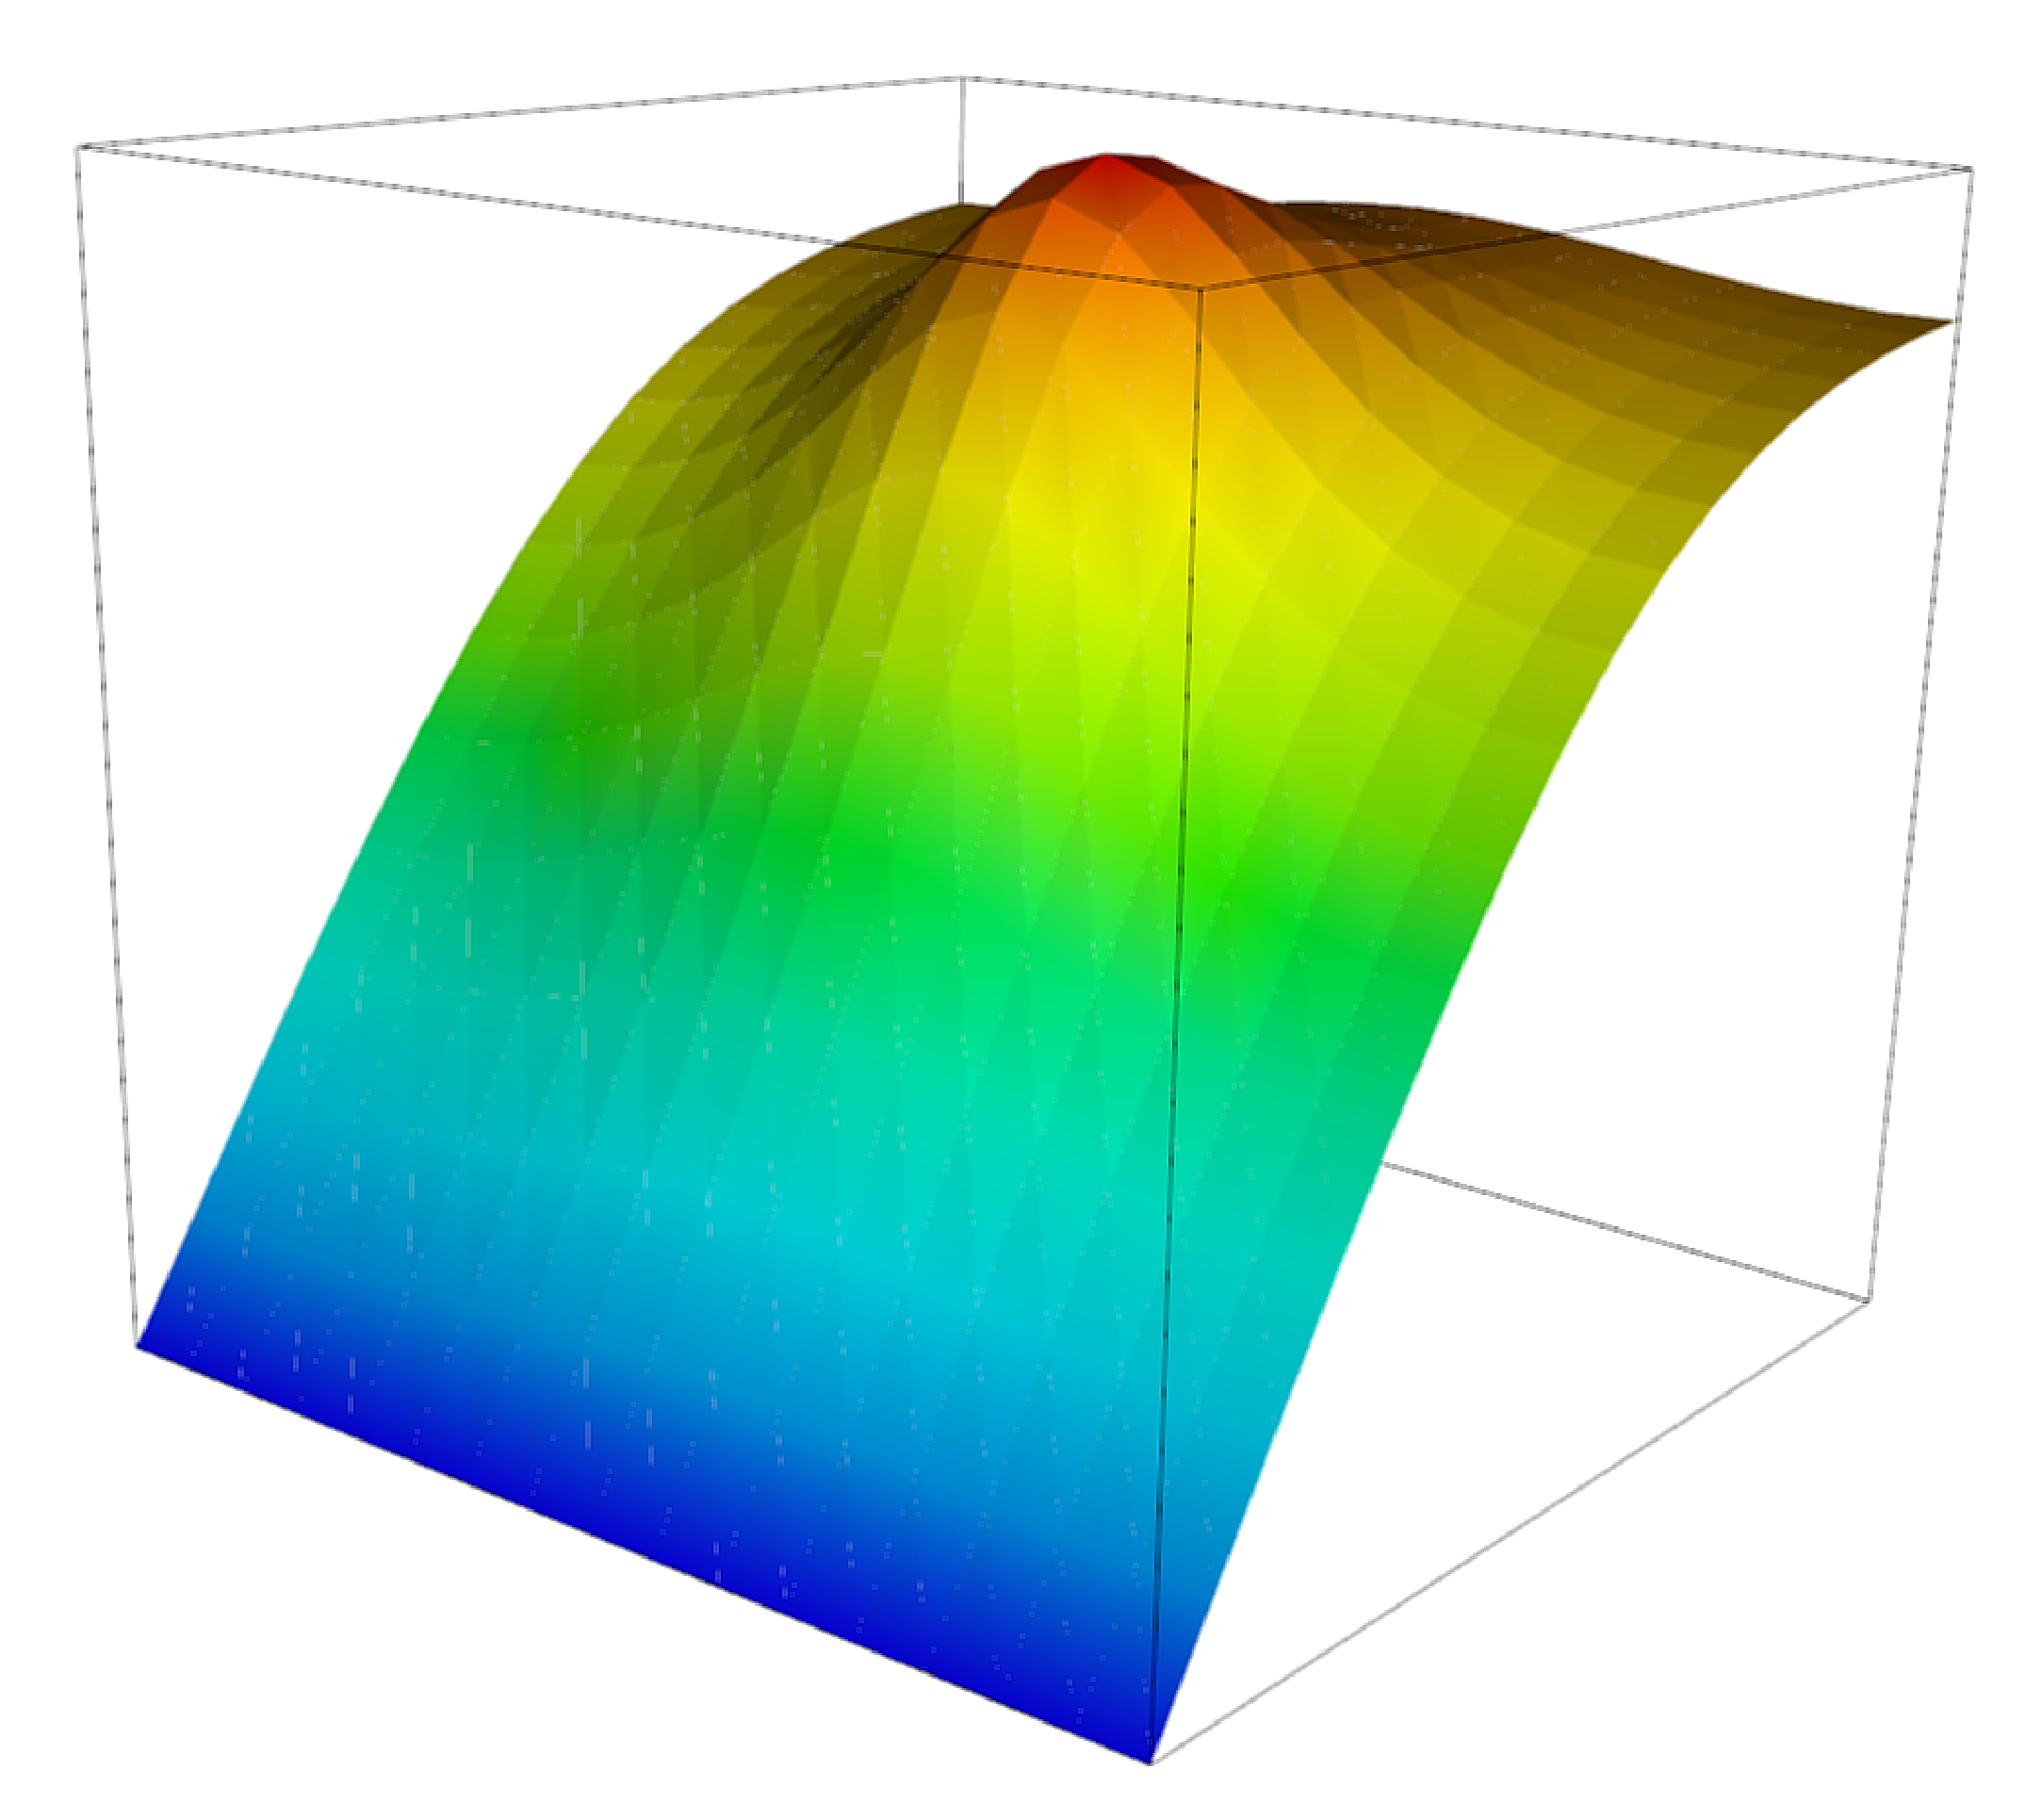
\includegraphics[width=10cm]{eps/poisson.eps}
    \caption{The solution of Poisson's equation (\ref{eq:poisson,quickstart})
      visualized in MayaVi.}
  \end{center}
\end{figure}
